\section{Descrizione Design Pattern} \label{app:design_pattern}

\subsection{Design Pattern Architetturali}

\subsubsection{MVC - Model View Controller}
\textit{Model-View-Controller} (MVC) è un pattern architetturale con la funzione di suddividere l'architettura dell'applicazione in tre parti distinte ma interconnesse, permettendo una separazione tra la gestione dei dati e la modalità attraverso la quale vengono mostrati all'utente.
I tre componenti sono:
\begin{itemize}
	\item \textbf{Model}: definisce il modello dei dati, ne realizza la logica e le diverse operazioni che possono essere effettuate su di essi. Viene progettato attraverso le tecniche object oriented e permette di notificare alle varie view l'aggiornamento del modello dei dati (Observer pattern).
	\item \textbf{View}: si occupa della gestione della logica di presentazione dei dati ai vari client, cattura gli input dell'utente e delega al controller la loro gestione. L'aggiornamento della view può avvenire in due modalità:
	\begin{itemize}
		\item \textbf{push model}: se la view deve essere costantemente aggiornata (Observer pattern); si usa se il pattern MVC si sviluppa in un unico ambiente di esecuzione;
		\item \textbf{pull model}: se la view necessita di essere aggiornata solo in momenti precisi; si usa se il pattern MVC si sviluppa su diversi ambienti di esecuzione.
	\end{itemize}
	\item \textbf{Controller}: trasforma le interazioni effettuate dal client attraverso la view in azioni sui dati presenti sul model. Ha la funzione di generare la logica dell'applicazione. Esiste un controller per ogni view.
\end{itemize}
MVC è fortemente utilizzato per applicazioni web.
\begin{figure}[H]
	\centering
	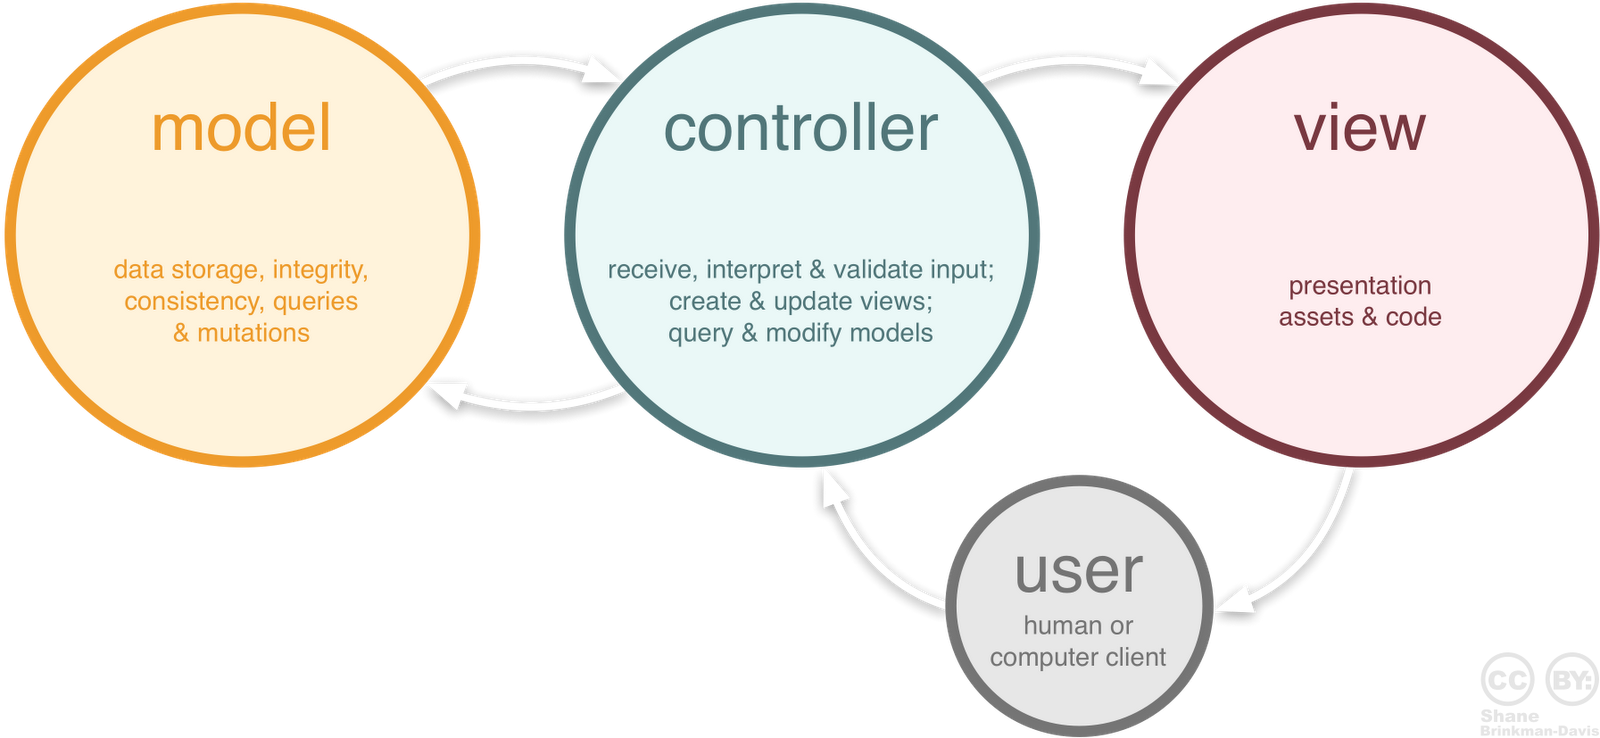
\includegraphics[width=14cm]{diagrammi_img/mvc.png}
	\caption{Design pattern MVC}
\end{figure}

\subsection{Design Pattern Creazionali}

\subsubsection{Singleton}
\textit{Singleton} è un pattern creazionale frequentemente utilizzato e necessario in molte applicazioni il cui scopo è di vincolare una classe alla creazione di una e una sola istanza della stessa, fornendo un punto di accesso unico e globale a questa istanza. Per permettere questo funzionamento è necessario fornire solo alla classe stessa la capacità di venire istanziata e di bloccarla nel caso questo sia già avvenuto. Il singleton dovrebbe essere estensibile utilizzando il subclassing.\\
Il pattern singleton garantisce le seguenti condizioni:
\begin{itemize}
	\item un accesso unico e controllato all'istanza, poiché solo la classe stessa è in grado di controllare l'accesso da parte dei client;
	\item l'istanza potrebbe essere usata come contenitore unico per variabili che altrimenti sarebbero globali;
	\item permette la definizione delle operazioni appartenenti alla classe che utilizza il singleton, la quale andrebbe sempre estesa prima dell'utilizzo;
	\item il numero delle istanze può essere controllato, e non è necessariamente limitato ad una sola. Questa funzione viene sempre gestita dalla classe stessa che implementa anche il modo di fornire ai vari client l'istanza corretta.
\end{itemize}

\begin{figure}
	\centering
	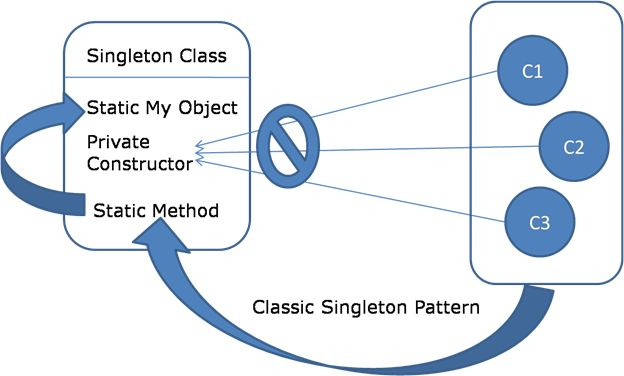
\includegraphics[width=10cm]{diagrammi_img/singleton.jpg}
	\caption{Modello concettuale del design pattern Singleton}
\end{figure}

\begin{figure}
	\centering
	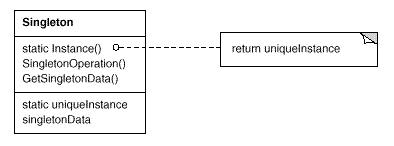
\includegraphics[width=10cm]{diagrammi_img/singleton_class.png}
	\caption{Design pattern Singleton}
\end{figure}

\subsection{Design Pattern Strutturali}

\subsubsection{Fa\c{c}ade}
\textit{Fa\c{c}ade} è un pattern strutturale che fornisce un'interfaccia unica per un insieme di sotto interfacce. La suddivisione del sistema in sottosistemi aiuta a ridurne la complessità.
Il pattern può essere utilizzato nei seguenti casi:
\begin{itemize}
	\item Per fornire un'interfaccia unica e semplificata ad un sottosistema complesso, che con la sua evoluzione tende ad aumentare di complessità, spesso a causa dell'utilizzo di altri pattern che rendono il sottosistema più riusabile e personalizzabile, ma rendono l'accesso dei client che non richiedono personalizzazione più complicato. Il fa\c{c}ade propone quindi una vista di default del sottosistema per chi non ha bisogno di un accesso dettagliato.
	\item Se vogliamo disaccoppiare i sottoinsiemi dai client a causa delle molte dipendenze introducendo un fa\c{c}ade queste possono essere ridotte, facilitandone la portabilità e l'indipendenza dei sottoinsiemi.
	\item Se abbiamo una struttura a più livelli e vogliamo organizzare i sottoinsiemi. Il fa\c{c}ade fa da punto di ingresso per i sottolivelli.
\end{itemize}

\begin{figure}[H]
	\centering
	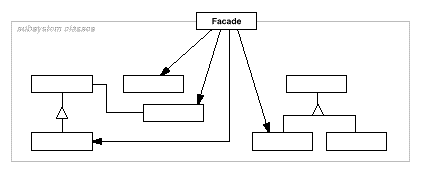
\includegraphics[width=10cm]{diagrammi_img/facade.png}
	\caption{Design pattern Facade}
\end{figure}

\subsubsection{Module}
Il \textit{module} pattern è un pattern tipico di JavaScript, utilizzato per incapsulare parti di oggetti.
Sfrutta la natura funzionale del linguaggio per ottenere lo scopo. Il module è una \glossario{Immediately-Invoked-Function-Expressions} (IIFE) al cui interno è possibile avere diversi tipi di accesso ai dati.
\begin{center}
	\begin{lstlisting}[language=JavaScript, caption=Design pattern Module]
		(function() {
			// declare private variables and/or functions
			return{
				// declare public variable and/or functions
			}
		})();
	\end{lstlisting}
\end{center}

\subsection{Design Pattern Comportamentali}

\subsubsection{Observer}
\textit{Observer} è un pattern comportamentale che definisce dipendenze uno a molti fra oggetti, riflettendo la modifica di uno di questi su tutti quelli a lui dipendenti. Questo permette di mantenere una consistenza tra gli oggetti in quanto il modello e le viste a lui collegate vengono aggiornate insieme. 
Il pattern definisce due ruoli:
\begin{itemize}
	\item \textbf{Subject}: colui che effettua le notifiche al variare dei dati;
	\item \textbf{Observer}: colui che si aggiorna alla ricezione delle notifiche.
\end{itemize}
Il pattern può essere utilizzato nei seguenti casi:
\begin{itemize}
	\item se si vogliono associare più viste differenti ad un'unica astrazione, aumentando il riuso dei singoli tipi;
	\item quando il cambiamento di stato di un oggetto provoca anche il cambiamento di altri e non si conosce quanti oggetti debbano cambiare;
	\item se si vuole evitare l'accoppiamento forte, si può notificare gli oggetti senza fare assunzioni su quali essi siano.
\end{itemize}

\begin{figure}[H]
	\centering
	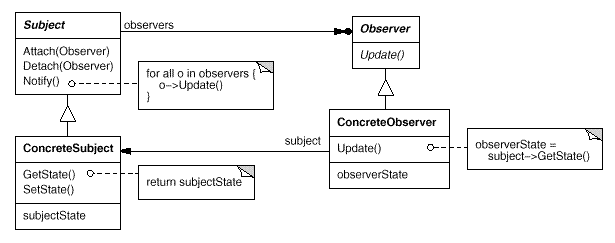
\includegraphics[width=14cm]{diagrammi_img/observer.png}
	\caption{Design pattern Observer}
\end{figure}